A conversão de sinais analógicos em processamento digital de sinais é fundamental em telecomunicações, redes de computadores, sistemas inteligentes, aplicações industriais, militares e governamentais. Isso se deve ao fato de que muitos sinais naturais, como grandezas físicas, são analógicos ou contínuos, e para que possam ser processados em dispositivos eletrônicos e computacionais, precisam ser convertidos para uma representação discreta. 

\begin{figure}[H]
    \centering
    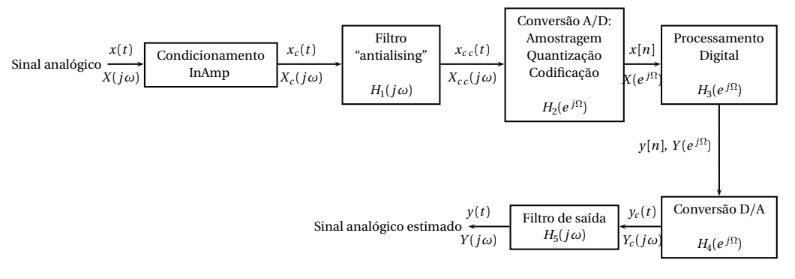
\includegraphics[width=1\linewidth]{image.png}
    \caption{Processamento a tempo discreto de sinais a tempo contínuo. Fonte: SANCA (2024)}
    \label{fig:enter-label}
\end{figure}
O processo de conversão analógico-digital (A/D) envolve três etapas principais: amostragem, quantização e codificação, sendo a amostragem o primeiro passo, onde valores discretos são capturados de um sinal originalmente contínuo no tempo.

A amostragem é crucial porque é nesse estágio que o sinal contínuo é transformado em uma sequência de pontos discretos que representará o sinal digitalmente. A qualidade dessa conversão afeta diretamente a precisão com que o sinal original pode ser reconstruído, evitando perdas de informação causadas por fenômenos como o \textit{aliasing}, que ocorre quando a taxa de amostragem é inadequada.

Neste trabalho, analisamos os princípios da amostragem por três métodos: ideal, natural e \textit{flat-top} (topo plano), com base no teorema da amostragem, e implementamos simulações computacionais para ilustrar os efeitos práticos da amostragem e reconstrução de sinais digitais. A simulação, baseada na modulação por amplitude de pulso (PAM) de um sinal senoidal puro, incluiu a análise do espectro de frequências, a aplicação de métodos de filtragem e a reconstrução do sinal original. Utilizamos a Transformada de Fourier (FT) para análise espectral, o teorema de Nyquist para determinar a taxa de amostragem adequada, e filtros passa-baixa para a reconstrução do sinal. O documento descreve detalhadamente cada etapa do processo, os teoremas aplicados, os cálculos realizados e as ferramentas computacionais utilizadas, além de apresentar os resultados obtidos.
